% Options for packages loaded elsewhere
\PassOptionsToPackage{unicode}{hyperref}
\PassOptionsToPackage{hyphens}{url}
\PassOptionsToPackage{dvipsnames,svgnames,x11names}{xcolor}
%
\documentclass[
]{ctexart}
\usepackage{amsmath,amssymb}
\usepackage{iftex}
\ifPDFTeX
  \usepackage[T1]{fontenc}
  \usepackage[utf8]{inputenc}
  \usepackage{textcomp} % provide euro and other symbols
\else % if luatex or xetex
  \usepackage{unicode-math} % this also loads fontspec
  \defaultfontfeatures{Scale=MatchLowercase}
  \defaultfontfeatures[\rmfamily]{Ligatures=TeX,Scale=1}
\fi
\usepackage{lmodern}
\ifPDFTeX\else
  % xetex/luatex font selection
\fi
% Use upquote if available, for straight quotes in verbatim environments
\IfFileExists{upquote.sty}{\usepackage{upquote}}{}
\IfFileExists{microtype.sty}{% use microtype if available
  \usepackage[]{microtype}
  \UseMicrotypeSet[protrusion]{basicmath} % disable protrusion for tt fonts
}{}
\makeatletter
\@ifundefined{KOMAClassName}{% if non-KOMA class
  \IfFileExists{parskip.sty}{%
    \usepackage{parskip}
  }{% else
    \setlength{\parindent}{0pt}
    \setlength{\parskip}{6pt plus 2pt minus 1pt}}
}{% if KOMA class
  \KOMAoptions{parskip=half}}
\makeatother
\usepackage{xcolor}
\usepackage[margin=1in]{geometry}
\usepackage{color}
\usepackage{fancyvrb}
\newcommand{\VerbBar}{|}
\newcommand{\VERB}{\Verb[commandchars=\\\{\}]}
\DefineVerbatimEnvironment{Highlighting}{Verbatim}{commandchars=\\\{\}}
% Add ',fontsize=\small' for more characters per line
\newenvironment{Shaded}{}{}
\newcommand{\AlertTok}[1]{\textcolor[rgb]{1.00,0.00,0.00}{\textbf{#1}}}
\newcommand{\AnnotationTok}[1]{\textcolor[rgb]{0.38,0.63,0.69}{\textbf{\textit{#1}}}}
\newcommand{\AttributeTok}[1]{\textcolor[rgb]{0.49,0.56,0.16}{#1}}
\newcommand{\BaseNTok}[1]{\textcolor[rgb]{0.25,0.63,0.44}{#1}}
\newcommand{\BuiltInTok}[1]{\textcolor[rgb]{0.00,0.50,0.00}{#1}}
\newcommand{\CharTok}[1]{\textcolor[rgb]{0.25,0.44,0.63}{#1}}
\newcommand{\CommentTok}[1]{\textcolor[rgb]{0.38,0.63,0.69}{\textit{#1}}}
\newcommand{\CommentVarTok}[1]{\textcolor[rgb]{0.38,0.63,0.69}{\textbf{\textit{#1}}}}
\newcommand{\ConstantTok}[1]{\textcolor[rgb]{0.53,0.00,0.00}{#1}}
\newcommand{\ControlFlowTok}[1]{\textcolor[rgb]{0.00,0.44,0.13}{\textbf{#1}}}
\newcommand{\DataTypeTok}[1]{\textcolor[rgb]{0.56,0.13,0.00}{#1}}
\newcommand{\DecValTok}[1]{\textcolor[rgb]{0.25,0.63,0.44}{#1}}
\newcommand{\DocumentationTok}[1]{\textcolor[rgb]{0.73,0.13,0.13}{\textit{#1}}}
\newcommand{\ErrorTok}[1]{\textcolor[rgb]{1.00,0.00,0.00}{\textbf{#1}}}
\newcommand{\ExtensionTok}[1]{#1}
\newcommand{\FloatTok}[1]{\textcolor[rgb]{0.25,0.63,0.44}{#1}}
\newcommand{\FunctionTok}[1]{\textcolor[rgb]{0.02,0.16,0.49}{#1}}
\newcommand{\ImportTok}[1]{\textcolor[rgb]{0.00,0.50,0.00}{\textbf{#1}}}
\newcommand{\InformationTok}[1]{\textcolor[rgb]{0.38,0.63,0.69}{\textbf{\textit{#1}}}}
\newcommand{\KeywordTok}[1]{\textcolor[rgb]{0.00,0.44,0.13}{\textbf{#1}}}
\newcommand{\NormalTok}[1]{#1}
\newcommand{\OperatorTok}[1]{\textcolor[rgb]{0.40,0.40,0.40}{#1}}
\newcommand{\OtherTok}[1]{\textcolor[rgb]{0.00,0.44,0.13}{#1}}
\newcommand{\PreprocessorTok}[1]{\textcolor[rgb]{0.74,0.48,0.00}{#1}}
\newcommand{\RegionMarkerTok}[1]{#1}
\newcommand{\SpecialCharTok}[1]{\textcolor[rgb]{0.25,0.44,0.63}{#1}}
\newcommand{\SpecialStringTok}[1]{\textcolor[rgb]{0.73,0.40,0.53}{#1}}
\newcommand{\StringTok}[1]{\textcolor[rgb]{0.25,0.44,0.63}{#1}}
\newcommand{\VariableTok}[1]{\textcolor[rgb]{0.10,0.09,0.49}{#1}}
\newcommand{\VerbatimStringTok}[1]{\textcolor[rgb]{0.25,0.44,0.63}{#1}}
\newcommand{\WarningTok}[1]{\textcolor[rgb]{0.38,0.63,0.69}{\textbf{\textit{#1}}}}
\usepackage{longtable,booktabs,array}
\usepackage{calc} % for calculating minipage widths
% Correct order of tables after \paragraph or \subparagraph
\usepackage{etoolbox}
\makeatletter
\patchcmd\longtable{\par}{\if@noskipsec\mbox{}\fi\par}{}{}
\makeatother
% Allow footnotes in longtable head/foot
\IfFileExists{footnotehyper.sty}{\usepackage{footnotehyper}}{\usepackage{footnote}}
\makesavenoteenv{longtable}
\usepackage{graphicx}
\makeatletter
\def\maxwidth{\ifdim\Gin@nat@width>\linewidth\linewidth\else\Gin@nat@width\fi}
\def\maxheight{\ifdim\Gin@nat@height>\textheight\textheight\else\Gin@nat@height\fi}
\makeatother
% Scale images if necessary, so that they will not overflow the page
% margins by default, and it is still possible to overwrite the defaults
% using explicit options in \includegraphics[width, height, ...]{}
\setkeys{Gin}{width=\maxwidth,height=\maxheight,keepaspectratio}
% Set default figure placement to htbp
\makeatletter
\def\fps@figure{htbp}
\makeatother
\setlength{\emergencystretch}{3em} % prevent overfull lines
\providecommand{\tightlist}{%
  \setlength{\itemsep}{0pt}\setlength{\parskip}{0pt}}
\setcounter{secnumdepth}{-\maxdimen} % remove section numbering
\ifLuaTeX
  \usepackage{selnolig}  % disable illegal ligatures
\fi
\usepackage{bookmark}

% User-friendly report settings
\usepackage{amsmath,amssymb,mathtools}
\usepackage{booktabs,longtable,array}
\usepackage{graphicx}
\usepackage{float}
\usepackage{tikz}
\usetikzlibrary{positioning,arrows.meta}
\usepackage{xurl}
\usepackage{fvextra}
\DefineVerbatimEnvironment{Highlighting}{Verbatim}{breaklines,commandchars=\\\{\}}
\DefineVerbatimEnvironment{verbatim}{Verbatim}{breaklines}
\setlength{\parskip}{0.55em}
\setlength{\parindent}{2em}
\renewcommand{\arraystretch}{1.18}

\IfFileExists{xurl.sty}{\usepackage{xurl}}{} % add URL line breaks if available
\urlstyle{same}
\hypersetup{
  pdftitle={L1-09 群时延 All-Pass 补偿算法行为级仿真报告},
  colorlinks=true,
  linkcolor={Maroon},
  filecolor={Maroon},
  citecolor={Blue},
  urlcolor={Blue},
  pdfcreator={LaTeX via pandoc}}

\title{L1-09 群时延 All-Pass 补偿算法行为级仿真报告}
\author{}
\date{}

\begin{document}
\maketitle

\section{L1-09 群时延 All-Pass
补偿算法行为级仿真报告}\label{l1-09-ux7fa4ux65f6ux5ef6-all-pass-ux8865ux507fux7b97ux6cd5ux884cux4e3aux7ea7ux4effux771fux62a5ux544a}

\subsection{摘要}\label{ux6458ux8981}

本文针对 L1-09 群时延补偿算法进行行为级仿真验证。L1-09 的目标是在 L1-08
完成幅频补偿后，继续针对链路中的 phase / group delay distortion
进行补偿，使系统在目标频带内的群时延更加平坦。当前实现采用多级二阶
all-pass IIR filter
作为补偿结构。该结构理论上不改变幅度响应，只改变相位响应，因此适合接在
L1-08 幅频 FIR 补偿之后，用于独立改善 phase / group delay 问题。

当前 pipeline 中，L1-09 的输入不是原始 H1，而是已经经过 L1-08
fixed-point FIR 后的响应：

\[
\mathrm{pre\_L1\_09\_response}(f)=H_1(f)\,H_{2,\mathrm{fixed}}(f)
\]

其中 H1 表示模拟硬件链路的复数频率响应，H2\_fixed 表示 L1-08 fixed-point
FIR 补偿器。L1-09 首先读取该复数响应中的相位，执行 unwrap 后计算 group
delay，再通过 least-squares 优化多级二阶 all-pass filter 的 pole radius
和 pole angle，使补偿后的 group delay 尽量接近常数。

在当前 clean full pipeline run \texttt{full\_combined\_20260605\_155348}
中，L1-09 前的 group delay ripple 为
\texttt{2.994724\ ns}；floating-point all-pass 补偿后降为
\texttt{2.108406\ ns}；fixed-point all-pass 补偿后为
\texttt{2.108794\ ns}。因此当前 L1-09 已经降低 group delay
ripple，但尚未完全拉平。fixed-point all-pass 的 pole
均位于单位圆内，\texttt{stable=True}，且
\texttt{saturation\_count=0}，说明当前系数量化后滤波器数值稳定。

git repo: \url{https://github.com/Yuzhe2005/L1-08-L1-09}

\begin{center}\rule{0.5\linewidth}{0.5pt}\end{center}

\subsection{1. 术语与缩略词}\label{ux672fux8bedux4e0eux7f29ux7565ux8bcd}

\begin{longtable}[]{@{}ll@{}}
\toprule\noalign{}
术语 & 含义 \\
\midrule\noalign{}
\endhead
\bottomrule\noalign{}
\endlastfoot
L1-08 & 幅频 FIR 补偿算法，主要补偿 magnitude ripple \\
L1-09 & 相位 / 群时延补偿算法，主要补偿 group delay ripple \\
H1 & 模拟硬件链路的复数频率响应 \\
H2 & L1-08 FIR 补偿器的频率响应 \\
H2\_fixed & fixed-point 量化后的 L1-08 FIR 频率响应 \\
all-pass filter & 幅度恒为 1、只改变相位的滤波器 \\
IIR & Infinite Impulse Response，无限冲激响应滤波器 \\
SOS & Second-Order Section，二阶滤波器 section \\
phase & 相位响应，单位 rad \\
unwrap & 去除 phase 中的 2π 跳变，使相位曲线连续 \\
group delay & 群时延，表示不同频率分量的传播延迟 \\
pole & IIR filter 分母多项式的根，决定反馈系统稳定性 \\
fixed-point & 固定 bit 宽的定点数表示 \\
saturation & 数值超过 fixed-point 可表示范围后被截断 \\
EVM & Error Vector Magnitude，误差向量幅度 \\
EVM\_LIN & 基于频率响应的线性 EVM 辅助指标 \\
QAM & Quadrature Amplitude Modulation，正交幅度调制 \\
\end{longtable}

\begin{center}\rule{0.5\linewidth}{0.5pt}\end{center}

\subsection{2.
问题背景与算法目标}\label{ux95eeux9898ux80ccux666fux4e0eux7b97ux6cd5ux76eeux6807}

\subsubsection{2.1 L1-09
需要解决的问题}\label{l1-09-ux9700ux8981ux89e3ux51b3ux7684ux95eeux9898}

真实硬件链路不仅会造成幅度不平坦，也会造成相位不线性。相位不线性的直接结果是
group delay
不平坦。对于宽带信号，不同频率分量如果经历不同延迟，最终叠加回时域时会发生波形畸变，从而影响调制信号质量。

L1-08 已经负责补偿幅频不平坦问题：

\[
\left|H_1(f)\,H_{2,\mathrm{fixed}}(f)\right|\ \text{尽量平坦}
\]

但是 L1-08 当前使用的是 real linear-phase FIR。它本身只引入近似常数
group delay，不负责主动修复 H1 中非线性相位造成的 group delay
ripple。因此 L1-09 需要在 L1-08 之后继续处理：

\begin{Shaded}
\begin{Highlighting}[]
\NormalTok{phase / group delay distortion}
\end{Highlighting}
\end{Shaded}

更准确地说，L1-09 当前分析和补偿的是：

\[
\mathrm{pre\_L1\_09\_response}(f)=H_1(f)\,H_{2,\mathrm{fixed}}(f)
\]

也就是信号已经通过 L1-08 fixed-point FIR 后，准备进入 L1-09
模块之前的复数响应。

\subsubsection{2.2 算法目标}\label{ux7b97ux6cd5ux76eeux6807}

L1-09 当前行为级仿真的目标包括：

\begin{enumerate}
\def\labelenumi{\arabic{enumi}.}
\tightlist
\item
  从 \texttt{H1\ *\ H2\_fixed} 的复数响应中提取相位。
\item
  对相位执行 unwrap，得到连续相位曲线。
\item
  根据连续相位计算 group delay。
\item
  使用多级二阶 all-pass IIR filter 产生额外的频率相关延迟。
\item
  使补偿后的 group delay 尽量接近常数。
\item
  对 all-pass 系数进行 fixed-point 量化。
\item
  检查量化后 IIR filter 的 pole 是否位于单位圆内。
\item
  使用 EVM\_LIN 和 QAM EVM 验证补偿前后的信号质量变化。
\end{enumerate}

当前阶段的重点是行为级算法验证，不是完整 RTL 级 fixed-point
仿真。也就是说，当前 fixed-point 主要量化 all-pass
系数并重新计算频率响应，尚未完整模拟每一级 IIR
运算中的乘法器、加法器、累加器、寄存器和逐级 rounding / saturation。

\begin{center}\rule{0.5\linewidth}{0.5pt}\end{center}

\subsection{3. 理论模型}\label{ux7406ux8bbaux6a21ux578b}

\subsubsection{3.1
复数频率响应}\label{ux590dux6570ux9891ux7387ux54cdux5e94}

硬件链路 H1 可以写成：

\[
H_1(f)=\left|H_1(f)\right|\exp\!\left(j\phi_{H1}(f)\right)
\]

其中：

\[
\begin{aligned}
\left|H_1(f)\right| &\quad \text{表示 magnitude response},\\
\phi_{H1}(f) &\quad \text{表示 phase response}.
\end{aligned}
\]

经过 L1-08 fixed-point FIR 后，进入 L1-09 之前的响应为：

\[
H_{\mathrm{pre}}(f)=H_1(f)\,H_{2,\mathrm{fixed}}(f)
\]

L1-09 关心的是 \texttt{Hpre(f)} 的 phase 和 group delay。

\subsubsection{3.2 Phase Unwrap}\label{phase-unwrap}

计算机中直接从复数响应得到的 phase 通常来自：

\[
\angle H_{\mathrm{pre}}(f)
\]

这个 phase 会被限制在：

\[
[-\pi,\ \pi]
\]

因此真实相位如果连续下降或上升超过 π，就会在图上出现突然跳变。unwrap
的作用是把这些人为的 \texttt{2π} 跳变去掉，让相位变成连续曲线。

例如 wrapped phase 可能类似：

\begin{Shaded}
\begin{Highlighting}[]
\NormalTok{2.9, 3.1, {-}3.0, {-}2.8}
\end{Highlighting}
\end{Shaded}

unwrap 后会变成：

\begin{Shaded}
\begin{Highlighting}[]
\NormalTok{2.9, 3.1, 3.283, 3.483}
\end{Highlighting}
\end{Shaded}

unwrap
不改变真实物理相位，只是把相位表示方式从``折叠形式''改成``连续形式''。这是计算
group delay 之前必须做的步骤, 避免对信号跳变求导。

\subsubsection{3.3 Group Delay 定义}\label{group-delay-ux5b9aux4e49}

group delay 定义为相位对角频率的负导数：

\[
\tau_g(f)=-\frac{d\phi(f)}{d\omega}
\]

其中：

\[
\omega=2\pi f
\]

如果相位是严格线性的：

\[
\phi(f)=-2\pi f\tau
\]

则 group delay 为常数：

\[
\tau_g(f)=\tau
\]

这表示所有频率分量经历同样的延迟，信号形状不会因为不同频率到达时间不同而被拉扯。反过来，如果
group delay
随频率起伏，就说明不同频率分量经历不同延迟，会造成宽带信号畸变。

\subsubsection{3.4 All-Pass Filter
的作用}\label{all-pass-filter-ux7684ux4f5cux7528}

all-pass filter 的核心特点是：

\[
\left|A\!\left(e^{j\Omega}\right)\right|=1
\]

也就是说，它不改变幅度，只改变相位：

\[
A\!\left(e^{j\Omega}\right)=\exp\!\left(j\phi_A(\Omega)\right)
\]

因此 all-pass filter 很适合接在 L1-08 后面：

\begin{Shaded}
\begin{Highlighting}[]
\NormalTok{L1{-}08: 主要改变 magnitude}
\NormalTok{L1{-}09: 主要改变 phase / group delay}
\end{Highlighting}
\end{Shaded}

L1-09 补偿后的响应可以写成：

\[
H_{\mathrm{out}}(f)=H_1(f)\,H_{2,\mathrm{fixed}}(f)\,A(f)
\]

由于 \texttt{\textbar{}A(f)\textbar{}\ =\ 1}，理论上：

\[
\left|H_{\mathrm{out}}(f)\right|=\left|H_1(f)\,H_{2,\mathrm{fixed}}(f)\right|
\]

所以 L1-09 不应该破坏 L1-08 已经完成的幅频补偿。

\subsubsection{3.5 二阶 All-Pass
Section}\label{ux4e8cux9636-all-pass-section}

当前程序使用多级二阶 all-pass section。单个二阶 all-pass section 写成：

\[
A_k(z)=
\frac{r_k^2-2r_k\cos(\theta_k)z^{-1}+z^{-2}}
{1-2r_k\cos(\theta_k)z^{-1}+r_k^2z^{-2}}
\]

其中：

\[
\begin{aligned}
r_k &\quad \text{pole radius},\\
\theta_k &\quad \text{pole angle}.
\end{aligned}
\]

分母决定 pole：

\[
1-2r_k\cos(\theta_k)z^{-1}+r_k^2z^{-2}=0
\]

它对应一对共轭 pole：

\[
\begin{aligned}
z &= r_k\exp(+j\theta_k),\\
z &= r_k\exp(-j\theta_k).
\end{aligned}
\]

所以 \texttt{r\_k} 决定 pole 离单位圆多远，\texttt{theta\_k} 决定该
section 主要作用在哪个频率附近。

\subsubsection{3.6 Pole 与稳定性}\label{pole-ux4e0eux7a33ux5b9aux6027}

IIR filter 有反馈项，因此稳定性由 pole 决定。对于数字 IIR filter：

\[
\begin{aligned}
\text{所有 pole 都在单位圆内} &\Rightarrow \text{stable},\\
\text{任意 pole 在单位圆外} &\Rightarrow \text{unstable}.
\end{aligned}
\]

单位圆内表示：

\[
|\mathrm{pole}|<1
\]

对于当前二阶 all-pass section：

\[
|\mathrm{pole}|=r_k
\]

因此只要：

\[
r_k<1
\]

该 section 就是稳定的。当前 fixed-point 检查中的 \texttt{stable=True}
衡量的正是所有量化后的 all-pass IIR pole 是否仍然位于单位圆内。

\subsubsection{3.7 多级 All-Pass
Cascade}\label{ux591aux7ea7-all-pass-cascade}

单个二阶 section 的补偿能力有限，因此当前 L1-09 使用多个 section 串联：

\[
A_{\mathrm{total}}(z)=A_1(z)A_2(z)\cdots A_N(z)
\]

当前 active 配置为：

\[
N=8
\]

串联后的总 phase 为各级 phase 之和：

\[
\phi_{A,\mathrm{total}}(f)=\sum_k \phi_{A,k}(f)
\]

总 group delay 也近似为各级 group delay 之和：

\[
\tau_{A,\mathrm{total}}(f)=\sum_k \tau_{A,k}(f)
\]

这使得 L1-09 可以通过多个局部 all-pass section 共同拟合复杂的 group
delay 补偿曲线。

\begin{center}\rule{0.5\linewidth}{0.5pt}\end{center}

\subsection{4.
行为级仿真方案设计}\label{ux884cux4e3aux7ea7ux4effux771fux65b9ux6848ux8bbeux8ba1}

\subsubsection{4.1 总体流程}\label{ux603bux4f53ux6d41ux7a0b}

当前 L1-09 pipeline 位于完整 L1-08 + L1-09 pipeline 的后半段：

\begin{center}
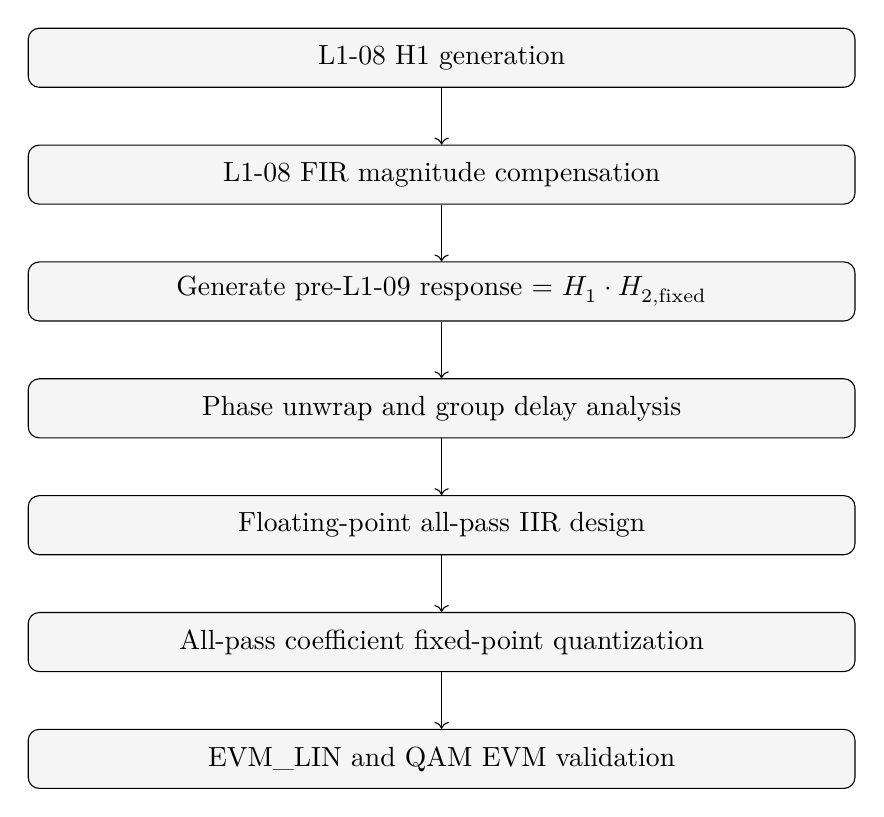
\begin{tikzpicture}[node distance=0.72cm, every node/.style={draw, rounded corners, align=center, minimum width=10.5cm, minimum height=0.75cm, fill=gray!8}]
\node (a) {L1-08 H1 generation};
\node (b) [below=of a] {L1-08 FIR magnitude compensation};
\node (c) [below=of b] {Generate pre-L1-09 response = $H_1\cdot H_{2,\mathrm{fixed}}$};
\node (d) [below=of c] {Phase unwrap and group delay analysis};
\node (e) [below=of d] {Floating-point all-pass IIR design};
\node (f) [below=of e] {All-pass coefficient fixed-point quantization};
\node (g) [below=of f] {EVM\_LIN and QAM EVM validation};
\foreach \i/\j in {a/b,b/c,c/d,d/e,e/f,f/g}{\draw[->] (\i) -- (\j);} 
\end{tikzpicture}
\end{center}

完整入口命令为：

\begin{Shaded}
\begin{Highlighting}[]
\OperatorTok{.}\FunctionTok{venv}\NormalTok{\textbackslash{}Scripts\textbackslash{}python}\OperatorTok{.}\FunctionTok{exe}\NormalTok{ run\_full\_l1\_08\_l1\_09\_pipeline}\OperatorTok{.}\FunctionTok{py}
\end{Highlighting}
\end{Shaded}

L1-09 单独入口为：

\begin{Shaded}
\begin{Highlighting}[]
\OperatorTok{.}\FunctionTok{venv}\NormalTok{\textbackslash{}Scripts\textbackslash{}python}\OperatorTok{.}\FunctionTok{exe}\NormalTok{ L1\_09\_sim\textbackslash{}run\_all\_l1\_09\_pipeline}\OperatorTok{.}\FunctionTok{py} \OperatorTok{{-}{-}}\NormalTok{run{-}dir }\KeywordTok{data}\NormalTok{\textbackslash{}}\OperatorTok{\textless{}}\NormalTok{run\_folder}\OperatorTok{\textgreater{}}
\end{Highlighting}
\end{Shaded}

\subsubsection{4.2 L1-09 程序结构}\label{l1-09-ux7a0bux5e8fux7ed3ux6784}

\begin{longtable}[]{@{}
  >{\raggedright\arraybackslash}p{(\columnwidth - 2\tabcolsep) * \real{0.5000}}
  >{\raggedright\arraybackslash}p{(\columnwidth - 2\tabcolsep) * \real{0.5000}}@{}}
\toprule\noalign{}
\begin{minipage}[b]{\linewidth}\raggedright
文件
\end{minipage} & \begin{minipage}[b]{\linewidth}\raggedright
功能
\end{minipage} \\
\midrule\noalign{}
\endhead
\bottomrule\noalign{}
\endlastfoot
\texttt{L1\_09\_group\_delay\_analyzer.py} & 读取 H1 和 L1-08 fixed FIR
响应，计算 \texttt{H1\ *\ H2\_fixed} 的 phase 和 group delay \\
\texttt{L1\_09\_allpass\_designer.py} & 设计 floating-point 多级二阶
all-pass IIR \\
\texttt{L1\_09\_fixed\_point\_quantizer.py} & 量化 all-pass
系数，检查稳定性并重新计算 fixed response \\
\texttt{L1\_09\_evm\_lin\_calculator.py} & 基于频率响应计算
EVM\_LIN、magnitude-only EVM 和 phase-only EVM \\
\texttt{L1\_09\_qam\_evm\_validator.py} & 用 QAM-loaded IF 信号验证
L1-09 前后 EVM 变化 \\
\texttt{run\_all\_l1\_09\_pipeline.py} & 串联运行完整 L1-09 pipeline \\
\texttt{L1\_09\_config.py} & 读取 L1-09 配置 \\
\end{longtable}

\subsubsection{4.3
数据输入与输出}\label{ux6570ux636eux8f93ux5165ux4e0eux8f93ux51fa}

当前项目目标输出规则为：

\begin{Shaded}
\begin{Highlighting}[]
\NormalTok{data/   保存 csv、json 等数据文件}
\NormalTok{graph/  保存 png 图像文件}
\end{Highlighting}
\end{Shaded}

一次 full pipeline 会生成：

\begin{Shaded}
\begin{Highlighting}[]
\NormalTok{data/full\_combined\_YYYYMMDD\_HHMMSS/}
\NormalTok{graph/full\_combined\_YYYYMMDD\_HHMMSS/}
\end{Highlighting}
\end{Shaded}

L1-09 主要输入包括：

\begin{Shaded}
\begin{Highlighting}[]
\NormalTok{data/\textless{}run\textgreater{}/h1\_full\_combined\_random/together.csv}
\NormalTok{data/\textless{}run\textgreater{}/l1\_08\_h2\_fixed\_point/h2\_fixed\_point\_response.csv}
\end{Highlighting}
\end{Shaded}

其中 \texttt{together.csv} 提供 H1 的 magnitude 和
phase，\texttt{h2\_fixed\_point\_response.csv} 提供 L1-08 fixed FIR
的频率响应。

L1-09 主要输出包括：

\begin{Shaded}
\begin{Highlighting}[]
\NormalTok{data/\textless{}run\textgreater{}/l1\_09\_fix\_group\_delay/group\_delay\_analysis.csv}
\NormalTok{data/\textless{}run\textgreater{}/l1\_09\_fix\_group\_delay/group\_delay\_metrics.csv}

\NormalTok{graph/\textless{}run\textgreater{}/l1\_09\_fix\_group\_delay/phase\_before\_l1\_09.png}
\NormalTok{graph/\textless{}run\textgreater{}/l1\_09\_fix\_group\_delay/group\_delay\_before\_l1\_09.png}
\NormalTok{graph/\textless{}run\textgreater{}/l1\_09\_fix\_allpass\_iir\_fs/allpass\_coefficients.csv}
\NormalTok{graph/\textless{}run\textgreater{}/l1\_09\_fix\_allpass\_iir\_fs/allpass\_response.csv}
\NormalTok{graph/\textless{}run\textgreater{}/l1\_09\_fix\_allpass\_iir\_fs/allpass\_metrics.csv}
\NormalTok{graph/\textless{}run\textgreater{}/l1\_09\_fix\_allpass\_iir\_fs/group\_delay\_before\_after\_l1\_09.png}
\NormalTok{graph/\textless{}run\textgreater{}/l1\_09\_fix\_allpass\_iir\_fixed/allpass\_coefficients\_fixed.csv}
\NormalTok{graph/\textless{}run\textgreater{}/l1\_09\_fix\_allpass\_iir\_fixed/allpass\_fixed\_response.csv}
\NormalTok{graph/\textless{}run\textgreater{}/l1\_09\_fix\_allpass\_iir\_fixed/allpass\_fixed\_metrics.csv}
\NormalTok{graph/\textless{}run\textgreater{}/l1\_09\_fix\_allpass\_iir\_fixed/allpass\_fixed\_quantization.png}
\NormalTok{graph/\textless{}run\textgreater{}/l1\_09\_fix\_evm\_lin\_fixed/evm\_lin.png}
\NormalTok{graph/\textless{}run\textgreater{}/l1\_09\_fix\_qam\_evm\_iir\_fixed/l1\_09\_qam\_evm.png}
\end{Highlighting}
\end{Shaded}

\begin{center}\rule{0.5\linewidth}{0.5pt}\end{center}

\subsection{5. All-Pass
设计方法}\label{all-pass-ux8bbeux8ba1ux65b9ux6cd5}

\subsubsection{5.1
为什么不能直接``提前''某些频率}\label{ux4e3aux4ec0ux4e48ux4e0dux80fdux76f4ux63a5ux63d0ux524dux67d0ux4e9bux9891ux7387}

真实物理系统不能让信号提前到达，只能增加延迟。因此 L1-09
的设计逻辑不是让慢的频率变快，而是让快的频率多等一会，使所有频率分量尽量接近同一个更晚的目标延迟。

程序中 target delay 的基本思想是：

\[
\mathrm{target\_delay\_ns}=\max(\mathrm{smoothed\_group\_delay\_ns})+\mathrm{margin\_ns}
\]

其中 \texttt{margin\_ns} 用于留出一点补偿余量。当前如果 config
中没有显式指定 margin，程序会使用：

\[
\mathrm{margin\_ns}=\max\left(0.05\ \mathrm{ns},\ 5\%\cdot\mathrm{original\_ripple\_ns}\right)
\]

当前 clean run 中：

\[
\begin{aligned}
\mathrm{target\_delay\_ns} &= 9.813229332\ \mathrm{ns},\\
\mathrm{target\_margin\_ns} &= 0.087111678\ \mathrm{ns}.
\end{aligned}
\]

\subsubsection{5.2 平滑处理}\label{ux5e73ux6ed1ux5904ux7406}

原始 group delay
中可能包含局部数值抖动。如果直接拟合所有尖锐抖动，all-pass filter
可能会过拟合，得到不够平滑或不够稳定的补偿结构。因此程序先使用 moving
average 对 group delay 进行平滑：

\[
\mathrm{fit\_delay\_ns}=\mathrm{moving\_average}(\mathrm{group\_delay\_ns},\ \mathrm{smooth\_window})
\]

当前配置：

\[
\mathrm{smooth\_window}=31
\]

需要注意，平滑只用于优化拟合目标；最终评估 compensated group delay
ripple 时仍然使用未平滑的原始 group delay 加上 all-pass group delay。

\subsubsection{5.3 优化变量}\label{ux4f18ux5316ux53d8ux91cf}

当前每个二阶 section 有两个主要参数：

\[
r_k,\quad \theta_k
\]

对于 N 个二阶 section，优化变量为：

\[
\left[r_1,r_2,\ldots,r_N,\theta_1,\theta_2,\ldots,\theta_N,\mathrm{target\_delay}\right]
\]

当前 active 配置：

\[
N=8
\]

因此需要优化 17 个量：

\[
8\ \text{个 } r,\quad 8\ \text{个 } \theta,\quad 1\ \text{个 target\_delay}
\]

\subsubsection{5.4 Least-Squares
目标函数}\label{least-squares-ux76eeux6807ux51fdux6570}

all-pass 产生的 group delay 记为：

\[
\tau_A(f)
\]

补偿后的 group delay 为：

\[
\tau_{\mathrm{comp}}(f)=\tau_{\mathrm{pre}}(f)+\tau_A(f)
\]

优化目标是让它尽量接近常数 \texttt{target\_delay}：

\[
\min \sum_f \left[\tau_{\mathrm{pre,smooth}}(f)+\tau_A(f)-\mathrm{target\_delay}\right]^2
\]

程序中为了数值稳定，会除以一个 scale：

\[
\mathrm{residual}(f)=
\frac{\tau_{\mathrm{pre,smooth}}(f)+\tau_A(f)-\mathrm{target\_delay}}
{\max(\mathrm{original\_ripple\_ns},\ 1.0)}
\]

该 scale 不改变优化目标的物理含义，只是让优化器中的数值量级更舒服。

\subsubsection{5.5 当前 All-Pass
设计结果}\label{ux5f53ux524d-all-pass-ux8bbeux8ba1ux7ed3ux679c}

当前 clean run 为：

\begin{Shaded}
\begin{Highlighting}[]
\NormalTok{full\_combined\_20260605\_155348}
\end{Highlighting}
\end{Shaded}

主要 all-pass 设计结果如下：

\begin{longtable}[]{@{}lr@{}}
\toprule\noalign{}
指标 & 数值 \\
\midrule\noalign{}
\endhead
\bottomrule\noalign{}
\endlastfoot
sampling rate & 12 GHz \\
all-pass section count & 8 \\
smooth window & 31 \\
original group delay ripple & 2.994724 ns \\
floating compensated group delay ripple & 2.108406 ns \\
compensated RMS to target & 0.364910 ns \\
optimizer success & True \\
\end{longtable}

代表性图像如下：

\begin{figure}
\centering
\IfFileExists{../graph/full_combined_20260605_155348/l1_09_fix_group_delay/group_delay_before_l1_09.png}{
\includegraphics{../graph/full_combined_20260605_155348/l1_09_fix_group_delay/group_delay_before_l1_09.png}}{\fbox{\parbox{0.86\linewidth}{\centering Image not found:\\ \ttfamily ../graph/full\_combined\_20260605\_155348/l1\_09\_fix\_group\_delay/group\_delay\_before\_l1\_09.png}}}
\caption{L1-09 group delay before compensation}
\end{figure}

\begin{figure}
\centering
\IfFileExists{../graph/full_combined_20260605_155348/l1_09_fix_allpass_iir_fs/group_delay_before_after_l1_09.png}{
\includegraphics{../graph/full_combined_20260605_155348/l1_09_fix_allpass_iir_fs/group_delay_before_after_l1_09.png}}{\fbox{\parbox{0.86\linewidth}{\centering Image not found:\\ \ttfamily ../graph/full\_combined\_20260605\_155348/l1\_09\_fix\_allpass\_iir\_fs/group\_delay\_before\_after\_l1\_09.png}}}
\caption{L1-09 group delay before and after all-pass compensation}
\end{figure}

\begin{center}\rule{0.5\linewidth}{0.5pt}\end{center}

\subsection{6. Fixed-Point 量化}\label{fixed-point-ux91cfux5316}

\subsubsection{6.1
当前系数量化格式}\label{ux5f53ux524dux7cfbux6570ux91cfux5316ux683cux5f0f}

当前 L1-09 all-pass filter 的系数量化格式为：

\begin{Shaded}
\begin{Highlighting}[]
\NormalTok{signed fixed{-}point Q3.15}
\end{Highlighting}
\end{Shaded}

对应：

\[
\begin{aligned}
\mathrm{total\_bits} &= 18,\\
\mathrm{frac\_bits} &= 15.
\end{aligned}
\]

量化步进为：

\[
\mathrm{LSB}=2^{-15}=0.000030517578125
\]

可表示范围约为：

\[
[-4.0,\ 3.999969482422]
\]

\subsubsection{6.2 软件中如何模拟 bit
精度}\label{ux8f6fux4ef6ux4e2dux5982ux4f55ux6a21ux62df-bit-ux7cbeux5ea6}

当前软件模拟 fixed-point 的方式是：

\begin{Shaded}
\begin{Highlighting}[]
\NormalTok{float coefficient}
\NormalTok{    ↓}
\NormalTok{除以 LSB}
\NormalTok{    ↓}
\NormalTok{round 到最近整数}
\NormalTok{    ↓}
\NormalTok{clip 到 fixed{-}point 可表示整数范围}
\NormalTok{    ↓}
\NormalTok{乘回 LSB，得到量化后的 coefficient}
\end{Highlighting}
\end{Shaded}

用公式表示：

\[
\begin{aligned}
q_{\mathrm{int}} &= \mathrm{round}\!\left(\frac{x}{\mathrm{LSB}}\right),\\
q_{\mathrm{int,clipped}} &= \mathrm{clip}(q_{\mathrm{int}},\ \mathrm{min\_int},\ \mathrm{max\_int}),\\
x_{\mathrm{fixed}} &= q_{\mathrm{int,clipped}}\cdot \mathrm{LSB}.
\end{aligned}
\]

其中：

\[
\mathrm{LSB}=2^{-\mathrm{frac\_bits}}
\]

当前这一步模拟的是``系数存储精度''，也就是 all-pass filter
的浮点系数如果被写进硬件寄存器，需要用有限 bit 表示时会发生什么误差。

\subsubsection{6.3 稳定性检查}\label{ux7a33ux5b9aux6027ux68c0ux67e5}

量化后，程序重新用 fixed coefficients 组成 SOS，并计算每一级 denominator
的 pole。判断条件为：

\[
\mathrm{max\_pole\_radius}<1\Rightarrow \mathrm{stable}=\mathrm{True}
\]

当前 clean run 中：

\begin{longtable}[]{@{}lr@{}}
\toprule\noalign{}
指标 & 数值 \\
\midrule\noalign{}
\endhead
\bottomrule\noalign{}
\endlastfoot
total bits & 18 \\
fraction bits & 15 \\
coefficient LSB & 3.0517578125e-05 \\
saturation count & 0 \\
max abs coefficient error & 1.520833e-05 \\
RMS coefficient error & 8.819765e-06 \\
max pole radius & 0.954581 \\
stable & True \\
\end{longtable}

这说明当前 Q3.15 系数量化后没有发生 saturation，pole
仍在单位圆内，all-pass IIR 数值稳定。

\subsubsection{6.4 Fixed-Point 后的 Group Delay
影响}\label{fixed-point-ux540eux7684-group-delay-ux5f71ux54cd}

当前 fixed-point 量化后，group delay ripple 与 floating-point
结果几乎一致：

\begin{longtable}[]{@{}lr@{}}
\toprule\noalign{}
指标 & 数值 \\
\midrule\noalign{}
\endhead
\bottomrule\noalign{}
\endlastfoot
original group delay ripple & 2.994724 ns \\
float compensated group delay ripple & 2.108406 ns \\
fixed compensated group delay ripple & 2.108794 ns \\
fixed vs float compensated GD RMS error & 0.000353 ns \\
fixed vs float compensated GD max error & 0.000869 ns \\
\end{longtable}

因此在当前 Q3.15 系数格式下，系数量化本身没有明显破坏 L1-09 的补偿效果。

\begin{figure}
\centering
\IfFileExists{../graph/full_combined_20260605_155348/l1_09_fix_allpass_iir_fixed/allpass_fixed_quantization.png}{
\includegraphics{../graph/full_combined_20260605_155348/l1_09_fix_allpass_iir_fixed/allpass_fixed_quantization.png}}{\fbox{\parbox{0.86\linewidth}{\centering Image not found:\\ \ttfamily ../graph/full\_combined\_20260605\_155348/l1\_09\_fix\_allpass\_iir\_fixed/allpass\_fixed\_quantization.png}}}
\caption{L1-09 fixed-point all-pass quantization}
\end{figure}

\subsubsection{6.5 当前 Fixed-Point
仿真的限制}\label{ux5f53ux524d-fixed-point-ux4effux771fux7684ux9650ux5236}

当前 fixed-point 仿真还不是完整 RTL 级 fixed-point。完整 RTL 级
fixed-point 还需要继续模拟：

\begin{Shaded}
\begin{Highlighting}[]
\NormalTok{input I/Q quantization}
\NormalTok{    ↓}
\NormalTok{每一级 all{-}pass filter 的乘法 fixed{-}point}
\NormalTok{    ↓}
\NormalTok{加法器 / accumulator fixed{-}point}
\NormalTok{    ↓}
\NormalTok{内部 delay register fixed{-}point}
\NormalTok{    ↓}
\NormalTok{每一级输出 rounding / truncation / saturation}
\NormalTok{    ↓}
\NormalTok{多级 SOS cascade 后的最终输出}
\end{Highlighting}
\end{Shaded}

当前阶段先验证了``系数量化后频率响应是否稳定、是否仍有补偿效果''。后续进入
RTL 设计时，需要把上述完整运算链条补进仿真模型。

\begin{center}\rule{0.5\linewidth}{0.5pt}\end{center}

\subsection{7. EVM 验证方法}\label{evm-ux9a8cux8bc1ux65b9ux6cd5}

\subsubsection{7.1 EVM\_LIN}\label{evm_lin}

EVM\_LIN 是基于频率响应的线性辅助指标。它不生成完整 QAM
时域波形，而是在频率响应上直接比较补偿前后相对于理想线性响应的误差。

当前程序会对以下三个 stage 计算 EVM\_LIN：

\begin{Shaded}
\begin{Highlighting}[]
\NormalTok{after\_h1}
\NormalTok{after\_l1\_08\_fixed\_fir}
\NormalTok{after\_l1\_08\_fixed\_fir\_plus\_l1\_09\_allpass}
\end{Highlighting}
\end{Shaded}

同时分解为：

\begin{Shaded}
\begin{Highlighting}[]
\NormalTok{evm\_lin\_percent}
\NormalTok{magnitude\_only\_evm\_percent}
\NormalTok{phase\_only\_evm\_percent}
\end{Highlighting}
\end{Shaded}

这种分解可以帮助判断误差主要来自幅度还是相位。

\subsubsection{7.2 QAM EVM}\label{qam-evm}

QAM EVM 是更接近通信信号的验证方式。它会生成 QAM-loaded IF 信号，经过
H1、L1-08 fixed FIR 和 L1-09 all-pass
后，比较输出星座点相对于参考星座点的误差。

当前 QAM 配置为：

\begin{Shaded}
\begin{Highlighting}[]
\NormalTok{qam\_order = 64}
\NormalTok{samples = 65536}
\NormalTok{freq\_min\_hz = 3.55 GHz}
\NormalTok{freq\_max\_hz = 4.45 GHz}
\NormalTok{qam\_seed = 703592441}
\end{Highlighting}
\end{Shaded}

QAM EVM 更接近系统行为，但也更受信号构造、频率 bin、fitted delay 和 gain
alignment 影响。

\begin{center}\rule{0.5\linewidth}{0.5pt}\end{center}

\subsection{8. 当前实验结果}\label{ux5f53ux524dux5b9eux9a8cux7ed3ux679c}

\subsubsection{8.1 Clean Run 设置}\label{clean-run-ux8bbeux7f6e}

本次报告引用的 clean run 为：

\begin{Shaded}
\begin{Highlighting}[]
\NormalTok{data/full\_combined\_20260605\_155348}
\NormalTok{graph/full\_combined\_20260605\_155348}
\end{Highlighting}
\end{Shaded}

主要 seed 为：

\begin{longtable}[]{@{}lr@{}}
\toprule\noalign{}
Seed 类型 & 数值 \\
\midrule\noalign{}
\endhead
\bottomrule\noalign{}
\endlastfoot
H1 seed & 911204371 \\
behavior seed & 1401186327 \\
QAM seed & 703592441 \\
\end{longtable}

L1-09 active 参数为：

\begin{longtable}[]{@{}lr@{}}
\toprule\noalign{}
参数 & 数值 \\
\midrule\noalign{}
\endhead
\bottomrule\noalign{}
\endlastfoot
all-pass sections & 8 \\
smooth window & 31 \\
margin ns & automatic \\
coefficient total bits & 18 \\
coefficient fractional bits & 15 \\
\end{longtable}

\subsubsection{8.2 Group Delay
补偿结果}\label{group-delay-ux8865ux507fux7ed3ux679c}

\begin{longtable}[]{@{}lr@{}}
\toprule\noalign{}
指标 & 数值 \\
\midrule\noalign{}
\endhead
\bottomrule\noalign{}
\endlastfoot
L1-09 输入 group delay mean & 4.113093 ns \\
L1-09 输入 group delay ripple & 2.994724 ns \\
floating all-pass 后 group delay ripple & 2.108406 ns \\
fixed all-pass 后 group delay ripple & 2.108794 ns \\
\end{longtable}

group delay ripple 降低量为：

\[
2.994724\ \mathrm{ns}-2.108794\ \mathrm{ns}=0.885930\ \mathrm{ns}
\]

相对改善约为：

\[
\frac{0.885930}{2.994724}=29.6\%
\]

因此当前 L1-09 确实降低了 group delay ripple，但补偿后仍有约
\texttt{2.109\ ns} 的 residual ripple，说明当前 8-section all-pass
只能部分拟合该 seed 下的 group delay distortion。

\subsubsection{8.3 EVM\_LIN 结果}\label{evm_lin-ux7ed3ux679c}

使用 fixed all-pass coefficients 时，EVM\_LIN 结果为：

\begin{longtable}[]{@{}
  >{\raggedright\arraybackslash}p{(\columnwidth - 6\tabcolsep) * \real{0.2000}}
  >{\raggedleft\arraybackslash}p{(\columnwidth - 6\tabcolsep) * \real{0.2667}}
  >{\raggedleft\arraybackslash}p{(\columnwidth - 6\tabcolsep) * \real{0.2667}}
  >{\raggedleft\arraybackslash}p{(\columnwidth - 6\tabcolsep) * \real{0.2667}}@{}}
\toprule\noalign{}
\begin{minipage}[b]{\linewidth}\raggedright
Stage
\end{minipage} & \begin{minipage}[b]{\linewidth}\raggedleft
EVM\_LIN
\end{minipage} & \begin{minipage}[b]{\linewidth}\raggedleft
Magnitude-only EVM
\end{minipage} & \begin{minipage}[b]{\linewidth}\raggedleft
Phase-only EVM
\end{minipage} \\
\midrule\noalign{}
\endhead
\bottomrule\noalign{}
\endlastfoot
after H1 & 11.614517\% & 1.769356\% & 11.374248\% \\
after L1-08 fixed FIR & 11.433072\% & 0.695221\% & 11.373721\% \\
after L1-08 fixed FIR + L1-09 all-pass & 1.185585\% & 0.242099\% &
1.160319\% \\
\end{longtable}

该结果说明：

\begin{enumerate}
\def\labelenumi{\arabic{enumi}.}
\tightlist
\item
  L1-08 主要降低 magnitude-only EVM。
\item
  L1-09 主要降低 phase-only EVM。
\item
  加入 L1-09 后，EVM\_LIN 从 \texttt{11.433072\%} 降到
  \texttt{1.185585\%}，改善明显。
\end{enumerate}

\begin{figure}
\centering
\IfFileExists{../graph/full_combined_20260605_155348/l1_09_fix_evm_lin_fixed/evm_lin.png}{
\includegraphics{../graph/full_combined_20260605_155348/l1_09_fix_evm_lin_fixed/evm_lin.png}}{\fbox{\parbox{0.86\linewidth}{\centering Image not found:\\ \ttfamily ../graph/full\_combined\_20260605\_155348/l1\_09\_fix\_evm\_lin\_fixed/evm\_lin.png}}}
\caption{L1-09 fixed EVM\_LIN}
\end{figure}

\subsubsection{8.4 QAM EVM 结果}\label{qam-evm-ux7ed3ux679c}

使用 fixed all-pass coefficients 时，QAM EVM 结果为：

\begin{longtable}[]{@{}lrr@{}}
\toprule\noalign{}
Stage & QAM EVM & Magnitude-only EVM \\
\midrule\noalign{}
\endhead
\bottomrule\noalign{}
\endlastfoot
after H1 & 11.733268\% & 1.633123\% \\
after L1-08 fixed FIR & 11.551006\% & 0.232999\% \\
after L1-08 fixed FIR + L1-09 all-pass & 3.396713\% & 2.263454\% \\
\end{longtable}

QAM EVM 从 \texttt{11.551006\%} 降到 \texttt{3.396713\%}，说明 L1-09
对相位相关失真有明显改善。但是 magnitude-only EVM 在加入 L1-09
后变大，这需要谨慎解释。

理论上 all-pass filter 幅度恒为 1，不应该改变 magnitude response。当前
QAM magnitude-only EVM 变大的原因可能是All pass filter 初始化的 past
output 如 y{[}n-1{]} (n = 0)
时设置成为0，也可能是其他原因，后续会意义判断

因此本报告对 QAM 结果的解读是：L1-09 明显降低整体 QAM EVM，但 QAM
magnitude-only 分量的变化还需要后续进一步验证。

\begin{figure}
\centering
\IfFileExists{../graph/full_combined_20260605_155348/l1_09_fix_qam_evm_iir_fixed/l1_09_qam_evm.png}{
\includegraphics{../graph/full_combined_20260605_155348/l1_09_fix_qam_evm_iir_fixed/l1_09_qam_evm.png}}{\fbox{\parbox{0.86\linewidth}{\centering Image not found:\\ \ttfamily ../graph/full\_combined\_20260605\_155348/l1\_09\_fix\_qam\_evm\_iir\_fixed/l1\_09\_qam\_evm.png}}}
\caption{L1-09 fixed QAM EVM}
\end{figure}

\begin{center}\rule{0.5\linewidth}{0.5pt}\end{center}

\subsection{9. 结论}\label{ux7ed3ux8bba}

当前 L1-09 行为级仿真已经完成从 group delay 分析、floating all-pass
设计、fixed-point 系数量化，到 EVM\_LIN / QAM EVM 验证的完整流程。

主要结论如下：

\begin{enumerate}
\def\labelenumi{\arabic{enumi}.}
\tightlist
\item
  L1-09 当前分析对象是 \texttt{H1\ *\ H2\_fixed}，也就是经过 L1-08
  fixed-point FIR 后进入 L1-09 之前的响应。
\item
  当前 8-section 二阶 all-pass IIR 可以降低 group delay
  ripple，但不能完全拉平。
\item
  本次 clean run 中，group delay ripple 从 \texttt{2.994724\ ns} 降到
  fixed-point 后的 \texttt{2.108794\ ns}。
\item
  fixed-point Q3.15 系数量化没有造成 coefficient saturation。
\item
  量化后 max pole radius 为 \texttt{0.954581}，所有 pole
  均位于单位圆内，因此 all-pass IIR 稳定。
\item
  EVM\_LIN 从 \texttt{11.433072\%} 降到 \texttt{1.185585\%}，说明 L1-09
  对 phase-only distortion 的补偿效果明显。
\item
  QAM EVM 从 \texttt{11.551006\%} 降到
  \texttt{3.396713\%}，说明行为级通信信号验证也显示整体改善。
\item
  当前 fixed-point 仍然是系数量化级别，不是完整 RTL 级 fixed-point
  运算仿真。
\end{enumerate}

综合来看，L1-09 当前算法方向是合理的，已经可以作为后续 sweep、RTL
fixed-point 建模和硬件实现讨论的基础。

\begin{center}\rule{0.5\linewidth}{0.5pt}\end{center}

\subsection{10. 后续工作}\label{ux540eux7eedux5de5ux4f5c}

后续建议按以下顺序继续：

\begin{enumerate}
\def\labelenumi{\arabic{enumi}.}
\tightlist
\item
  增加 L1-09 sweep，覆盖 all-pass section count、fixed-point
  format、seed case 和 bandwidth profile。
\item
  对比 6、8、10 个 all-pass section 在不同 H1 phase distortion
  下的稳定性和补偿效果。
\item
  当前 QAM magnitude-only 经过 L1-08+L1-09 增大的结果。
\item
  建立完整 RTL 级 fixed-point 仿真，包括 I/Q input
  quantization、乘法器、加法器、accumulator、delay register 和逐级
  rounding / saturation。
\item
  将 L1-08 和 L1-09 的指标统一汇总，包括 magnitude ripple、group delay
  ripple、EVM\_LIN、QAM EVM 和 fixed-point stability。
\end{enumerate}

\end{document}
